\section{The ANNs }
The Artificial Neural Network used for this project was a modified ANN from Dr. Pyeatte's code. We converted his ANN to python and removed the back-propagation function and saving and loading from files. We added a mutation function and a recombination function. The mutation function takes the number of weights that are to be mutated then randomly chooses that number of weights and randomly assigns them a value. The recombination function takes to lists of weights as arguments and gives a 50-50 chance of choosing a weight from one or the other to create its own weights.

See Figure~\ref{systemdiagram}.  This is an example of a building phase ANN. The whole game board is given as inputs to the neural network. The number of colonists, each building and plantation type, number of each resource, victory points, and the amount of dabloons they have are all given under the player inputs. Player1 inputs used to save space in the figure. All of this information fed through the hidden layers and then outputs in the building phase are ranked. The higher the output the better the option is. The player will start with the best ranked option and try to do it. If it doesn't have enough dabloons to buy it the next option is chosen and repeats until something is bought or buy nothing is chosen.
\begin{figure}[tbh]
\begin{center}
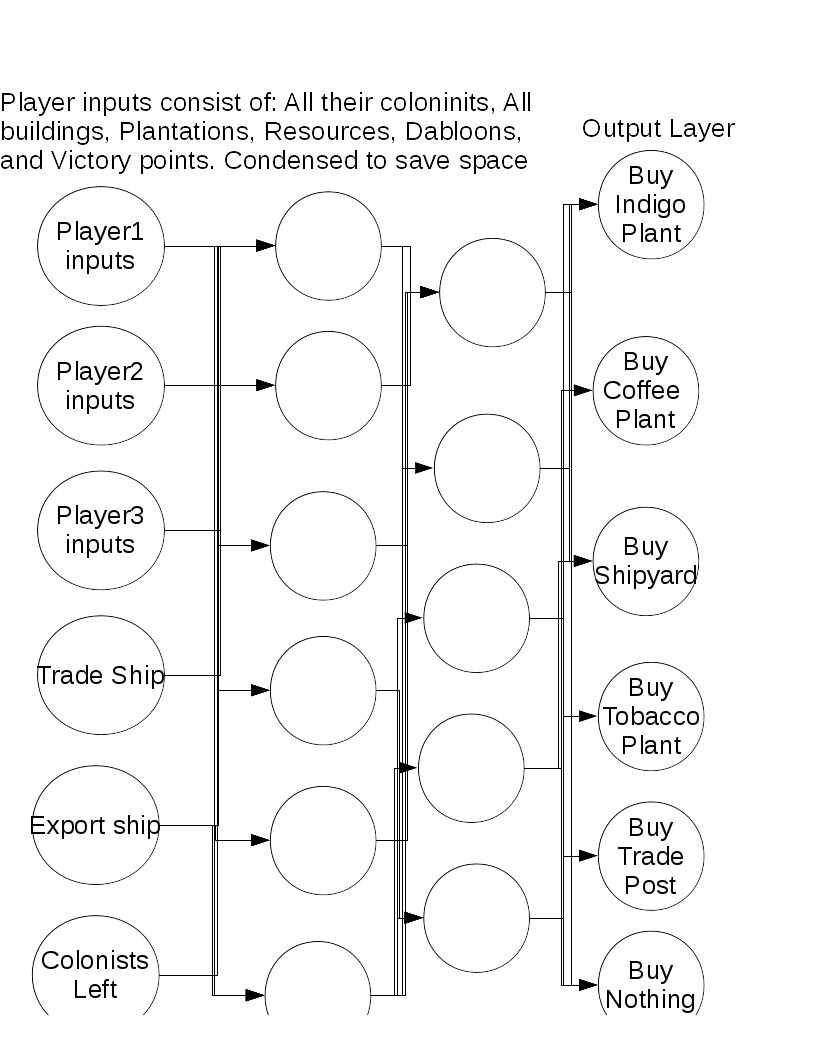
\includegraphics[width=0.75\textwidth]{./images/Example_ANN.png}
\end{center}
\caption{A example of a building phase ANN \label{systemdiagram}}
\end{figure}

\begin{algorithm} [tbh]                     % enter the algorithm environment
\caption{Calculate $y = x^n$}          % give the algorithm a caption
\label{alg1}                           % and a label for \ref{} commands later in the document
\begin{algorithmic}                    % enter the algorithmic environment
    \REQUIRE $n \geq 0 \vee x \neq 0$
    \ENSURE $y = x^n$
    \STATE $y \Leftarrow 1$
    \IF{$n < 0$}
        \STATE $X \Leftarrow 1 / x$
        \STATE $N \Leftarrow -n$
    \ELSE
        \STATE $X \Leftarrow x$
        \STATE $N \Leftarrow n$
    \ENDIF
    \WHILE{$N \neq 0$}
        \IF{$N$ is even}
            \STATE $X \Leftarrow X \times X$
            \STATE $N \Leftarrow N / 2$
        \ELSE[$N$ is odd]
            \STATE $y \Leftarrow y \times X$
            \STATE $N \Leftarrow N - 1$
        \ENDIF
    \ENDWHILE
\end{algorithmic}
\end{algorithm}
